\section{Experimental Results}
For our evaluation, we implemented PC extractor module at the 
system call layer 
and PC-Lifetime analyzer and PC-to-Stream mapper module 
at the block device layer in the Linux kernel version 4.5.

In order to evaluate the effectiveness of {\sf PCStream},
we implemented the multi-stream feature and substream concept
to the in-house SSD emulator
based on the open flash development platform~\cite{AMF}.
The number of streams was set to 8 for the evaluation.
The SSD emulator was 8 GB with four channels with four ways, and 
the number of blocks per a parallel unit was 512 and
the number of pages per block was 256 with 4KB-sized page.
Due to the limited capacity of the emulator, 
we scaled down RocksDB configuration.
The base file size is set to 8 MB
with the size of key-value is 8 KB and the number of levels was set to 4.
However, the size of level multiplier is remained to be 10 as an usual setting,
which means the size of the next level is 10 times larger than previous level,
to maintain the level access patterns during the compaction.

For benchmarks, we used three scenarios of db\_bench of RocksDB.
The update random scenario (read-modify-write for random keys), {\tt UR}, and 
the append random scenario (read-modify-write with growing values), {\tt AR}, are
for intensively updating key-value pairs.
For each scenario, about 900000 keys are inserted.
The fill random scenario (write values in random key order), {\tt FR}, 
inserts 300000 key-value pairs 
after 70\% of the device capacity was filled.

For the comparison, 
we also implemented Autostream, manual technique, and
baseline which does not use the stream allocation policy.
We compared WAF of the existing techniques with {\sf PCStream}
for each scenario.

\begin{figure}[t]
	\centering
	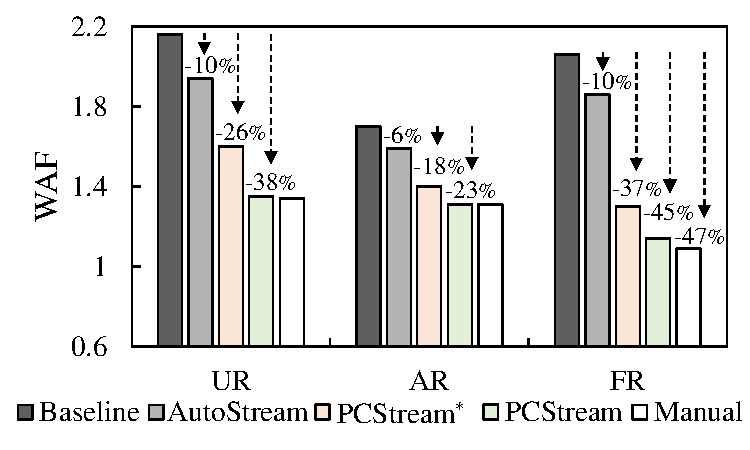
\includegraphics[width=0.8\linewidth]{figure/result_emul}
	\vspace{-10pt}
	\caption{The WAF comparison on the emulator.}
	\label{fig:result_emul}
	\vspace{-15pt}
\end{figure}

As shown in Fig.~\ref{fig:result_emul}, 
{\sf PCStream} reduces WAF by up to 45\% over the baseline technique. 

In order to evaluate the effectiveness of {\sf PCStream},
we used Samsung PM963 480GB SSD (with 8 streams).
As a warming workload, we wrote a single file sequentially to fill 90\%
of logical device capacity, to ensure that 90\% of logical space stays valid
throughout the test.

\begin{figure}[t]
	\centering
	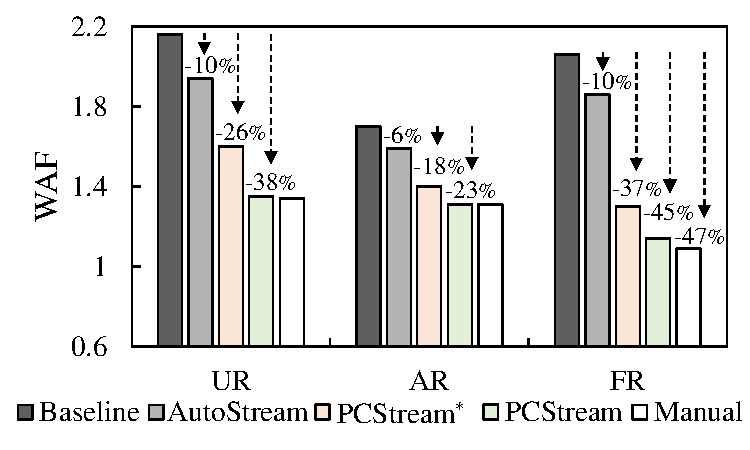
\includegraphics[width=0.8\linewidth]{figure/result_emul}
	\vspace{-10pt}
	\caption{The WAF comparison on the SSD.(temporarily placed to check paper length)}
	\label{fig:result_SSD}
	\vspace{-15pt}
\end{figure}


